%%=============================================================================
%% Methodologie
%%=============================================================================

\chapter{\IfLanguageName{dutch}{Methodologie}{Methodology}}%
\label{ch:methodologie}

%% TODO: In dit hoofstuk geef je een korte toelichting over hoe je te werk bent
%% gegaan. Verdeel je onderzoek in grote fasen, en licht in elke fase toe wat
%% de doelstelling was, welke deliverables daar uit gekomen zijn, en welke
%% onderzoeksmethoden je daarbij toegepast hebt. Verantwoord waarom je
%% op deze manier te werk gegaan bent.
%% 
%% Voorbeelden van zulke fasen zijn: literatuurstudie, opstellen van een
%% requirements-analyse, opstellen long-list (bij vergelijkende studie),
%% selectie van geschikte tools (bij vergelijkende studie, "short-list"),
%% opzetten testopstelling/PoC, uitvoeren testen en verzamelen
%% van resultaten, analyse van resultaten, ...
%%
%% !!!!! LET OP !!!!!
%%
%% Het is uitdrukkelijk NIET de bedoeling dat je het grootste deel van de corpus
%% van je bachelorproef in dit hoofstuk verwerkt! Dit hoofdstuk is eerder een
%% kort overzicht van je plan van aanpak.
%%
%% Maak voor elke fase (behalve het literatuuronderzoek) een NIEUW HOOFDSTUK aan
%% en geef het een gepaste titel.

Volgende hoofdstukken verlopen in sequentiële volgorde om dit onderzoek in de juiste richting te sturen.
De literatuurstudie geeft een basis om verdere vakterminologie en werking van technologieën te kunnen begrijpen.
\\
De setup van het huidige systeem wordt besproken om de requirements te kunnen begrijpen.
Het bekomen van een shortlist wordt toegelicht waarbij voor elke technologie de voor- en nadelen wordt beschreven.


\section{Phase 1: Literatuurstudie}
Voor dit onderzoek heb ik eerst de vaktermen opgelijst en onderverdeeld in groepen met behulp van een mindmap.
Vervolgens werd er gebruik gemaakt van het internet om wetenschappelijke artikelen op te zoeken en filterde ik de nodige informatie.
\\
Het doel van de literatuurstudie is om een basis van bestaande kennis te verkrijgen door de belangrijkste concepten toe te lichten die van toepassing zijn op dit onderzoek. 
Dit houd in, het begrijpen van warehousing, WCS (Warehouse Control Systems), PLC (Programmable Logic Controllers), en de communicatieprotocollen die tussen deze systemen gebruikt worden.
\\
Hierdoor krijg je een overzicht van relevante theorieën, definities, en eerdere studies die inzicht geven in de werking en de gebruikte technologieën.
Hier werd voornamelijk gebruik gemaakt van wetenschappelijke artikelen, boeken en technische documenten.
\\
De literatuurstudie vormt de basis van het onderzoek en is cruciaal voor het begrijpen van de huidige stand van zaken.
Hierdoor kan de kennis en requirements meegenomen worden doorheen de methodologie.

\section{Phase 2: Long List}
In dit hoofdstuk vertrekken we van een lijst met message brokers die beschikbaar zijn op de markt.
Deze worden kort besproken en later gefilterd door bepaalde criteria toe te passen, waarna de overgebleven kandidaten getest worden.
Op deze manier worden alle mogelijke opties geargumenteerd.

\subsection{Beschikbare messaging software}

\begin{table}[h!]
\footnotesize
\centering
\begin{tabular}{|l|c|c|c|c|c|}
\hline
Message Broker & JMS & Linux & Protocollen & Kostenmodel & On premise \\
\hline
Apache Kafka & Ja & Ja & Kafka, MQTT, REST & Open-source & Ja \\
\hline
RabbitMQ & Ja & Ja & AMQP, MQTT, STOMP & Open-source & Ja \\
\hline
ActiveMQ & Ja & Ja & AMQP, MQTT, STOMP, OpenWire & Open-source & Ja \\ 
\hline
Artemis & Ja & Ja & AMQP, MQTT, STOMP & Open-source & Ja \\
\hline
MQTT.js & Ja & Ja & MQTT & Open-source & Ja \\
\hline
IBM MQ & Ja & Ja & MQ, MQTT & Abonnement & Ja \\
\hline
Redis & Ja & Ja & Stream, Pub/Sub & Open-source & Ja \\
\hline
NSQ & Ja & Ja & Stream, Pub/Sub & Open-source & Ja \\
\hline
Apache Pulsar & Ja & Ja & Stream, Pub/Sub & Open-source & Ja \\
\hline
NATS & Ja & Ja & NATS & Open-source & Ja \\
\hline
ZeroMQ & Ja & Ja & ØMQ (Socket) & Open-source & Ja \\ 
\hline
Amazon SQS & Nee & Nee & AWS protocol & Pay-per-use & Nee \\
\hline
Google Cloud Pub/Sub & Nee & Nee & Cloud Pub/Sub & Pay-per-use & Nee \\
\hline
Azure Service Bus & Nee & Nee & AMQP, MQTT, HTTP & Pay-per-use & Nee \\
\hline
Solace PubSub+ & Ja & Nee & AMQP & Pay-per-use & Nee \\
\hline
\end{tabular}
\caption{\label{tab:message_brokers}Longlist message brokers}
\end{table}

\subsubsection{Apache Kafka}
Apache Kafka beschikt over een grote en actieve community waarvan diverse bedrijven betaalde ondersteuning aanbieden.
Kafka wisselt data uit via streams en ondersteunt geen AMQP-protocol. 
Communicatie met Kafka is mogelijk via een Kafka-adapter in Progress OpenEdge 12.8.
Aangezien het WCS draait op Progress OpenEdge 11.7, is Kafka niet compatibel met de huidige setup.
Hierdoor voldoet deze broker niet aan de gestelde requirements en kan deze niet als optie worden gekozen.
Ondanks deze technologie momenteel niet kan gebruikt worden, kan het wel een kandidaat zijn in de toekomst.

\subsubsection{RabbitMQ}
RabbitMQ is een open source message broker die geïnstalleerd kan worden op diverse Linux-distributies en een breed scala aan mogelijkheden biedt.
Deze broker ondersteunt functies zoals routering, filtering, streaming, en meer.
Routering naar queues is mogelijk via verschillende protocollen, waaronder AMQP, wat RabbitMQ zeer veelzijdig maakt.
Daarnaast beschikt RabbitMQ over uitgebreide documentatie, actieve ontwikkeling, een grote community, en de mogelijkheid tot professionele ondersteuning.
Omdat RabbitMQ JMS-ondersteuning biedt, is het geschikt voor onze shortlist en voldoet het aan de gestelde eisen.

\subsubsection{ActiveMQ Classic}
ActiveMQ Classic is een populaire JMS-gebaseerde message broker met een grote en actieve community.
Het kan eenvoudig worden geïnstalleerd in zowel lokale als cloudomgevingen en functioneert uitstekend op moderne Linux-systemen.
De broker ondersteunt meerdere protocollen, waaronder AMQP, naast OpenWire, STOMP, en MQTT, wat het veelzijdig maakt in uiteenlopende toepassingen.
Daarnaast is ActiveMQ Classic gratis en vereist het geen licentiekosten, wat het bijzonder aantrekkelijk maakt voor bedrijven met een beperkt budget.
Hoewel ActiveMQ Classic een stabiele en bewezen oplossing is, verschuift het momentum van de community langzaam richting ActiveMQ Artemis, 
waardoor toekomstige innovaties minder frequent kunnen zijn.
Desondanks blijft het een betrouwbare keuze voor organisaties die op zoek zijn naar een kostenbesparende en robuuste message broker.

\subsubsection{ActiveMQ Artemis}
ActiveMQ Artemis is een open source JMS-gebaseerde broker, vergelijkbaar met ActiveMQ Classic, maar met een andere interne architectuur.
Artemis gebruikt een eigen opslagmechanisme dat sneller is dan KahaDB, de opslaglaag die door ActiveMQ Classic wordt gebruikt.
Berichten worden sequentieel opgeslagen, waardoor er geen aparte index nodig is.
Dit vermindert de kans op prestatieverlies, zelfs bij het verwerken van grote hoeveelheden berichten.
De broker ondersteunt verschillende protocollen, waaronder AMQP, waardoor Artemis geschikt is voor diverse toepassingen.
Zowel community support als commerciële ondersteuning via verschillende bedrijven is beschikbaar, 
wat flexibiliteit biedt in onderhoud en beheer.

\subsubsection{MQTT.js}
MQTT.js is een open source JavaScript library voor het implementeren van het MQTT-protocol in zowel Node.js- als browseromgevingen.

Bron: https://github.com/mqttjs

\subsubsection{IBM MQ}
IBM MQ is een JMS-gebaseerde message broker en is geschikt voor Linux OS-omgevingen en kan draaien op zowel on-premises als cloud omgevingen.
IBM MQ ondersteunt meerdere protocollen, waaronder AMQP, wat het flexibel maakt in hybride omgevingen waar interoperabiliteit met verschillende systemen vereist is.
De broker biedt enterprise-grade functionaliteit met ondersteuning voor transacties, garanties voor berichtlevering, en beveiliging, wat het ideaal maakt voor veeleisende toepassingen.
Wat betreft het kostenmodel biedt IBM MQ licentiemodellen op basis van vier categorieën, 
met verschillende opties voor zowel lokale implementaties als cloud gebaseerde oplossingen.
Naast de betalende versie is er ook een gratis proef versie.
De kosten kunnen relatief hoog zijn, maar biedt wel uitgebreide functionaliteiten en garanties.
IBM MQ heeft een gesloten community en biedt ondersteuning via IBM zelf. 
Dit maakt het een goede keuze voor organisaties die behoefte hebben aan robuuste, goed ondersteunde messaging-oplossingen.
Voor het WCS kan deze technologie als overmatig gezien worden omdat de vele functionaliteiten niet toegepast worden.

\subsubsection{Redis}
Redis is een in-memory data platform dat kan gebruikt worden als message broker dat gebruik maakt van streams of pub/sub via API. 
Het ondersteunt JMS enkel maar via verschillende client bibliotheken en is compatibel met Linux OS-omgevingen, 
wat het geschikt maakt voor zowel lokale als cloud implementaties.
Hoewel Redis oorspronkelijk geen specifiek messaging-protocol zoals AMQP ondersteunt, 
kan het berichtenuitwisseling realiseren via pub/sub-mechanismen. 
Wat betreft het kostenmodel, Redis is open source en gratis te gebruiken, wat het aantrekkelijk maakt voor organisaties met beperkte budgetten. 
Redis biedt ook cloud-gebaseerde services via aanbieders zoals Redis Labs, met premium opties voor extra functionaliteit en ondersteuning.
De community rond Redis is groot en actief, met veel beschikbare documentatie, tutorials en third-party tools. 
Voor bedrijven die commerciële ondersteuning nodig hebben, biedt Redis Labs betaalde ondersteuning en aanvullende services, waaronder geavanceerde beveiliging en schaalbaarheid.

\subsubsection{NSQ}
NSQ is een open source, gedistribueerde message broker die ontworpen is voor hoge beschikbaarheid en schaalbaarheid. 
JMS-integratie is enkel geschikt via client libraries van NSQ.
Deze software werkt op Linux OS-omgevingen, wat het geschikt maakt voor zowel lokale als cloud gebaseerde implementaties.
NSQ is ontworpen om berichtenverkeer op grote schaal te verwerken en biedt geen AMQP-protocol, enkel ondersteuning voor pub/sub-communicatie. 
Het kostenmodel van NSQ is open source en volledig gratis te gebruiken. 
Er zijn geen licentiekosten, en de schaalbaarheid van het systeem maakt het geschikt voor zowel kleine als grote omgevingen.
NSQ heeft een actieve community die regelmatig updates en ondersteuning biedt via GitHub en andere open source platforms. 
Voor bedrijven die behoefte hebben aan commerciële ondersteuning, zijn er diverse consultants en serviceproviders die ondersteuning bieden.

\subsubsection{Apache Pulsar}
Apache Pulsar is een project gestart door Yahoo en open source sinds 2016.
Dit is een gedistribueerde messaging systeem dat ondersteuning biedt voor zowel streaming en messaging en wordt gezien als een "all-in-one" oplossing.
Het vooral bedoeld voor cloud omgevingen maar is ook geschikt voor lokale omgevingen.
AMQP kan gebruikt worden via een connector maar brengt hierdoor extra complexiteit met zich mee.
Deze software wordt gebruikt voor meer complexere use-cases waar elasticiteit en horizontale uitbreiding nodig is
en heeft daardoor een ingewikkelde setup.
De community rondom Apache Pulsar is actief, met regelmatige updates en ondersteuning via de Apache Software Foundation. 
Commerciële ondersteuning is beschikbaar via bedrijven die Pulsar als platform aanbieden.
\\\\
Bron: https://www.baeldung.com/apache-pulsar

\subsubsection{NATS}
NATS is een open source messaging systeem dat gebruik maakt van het NATS protocol. Dit omvat TCP, MQTT en Socket.
Dit protocol gebruikt het publish-subscribe-model en geeft dus geen ondersteuning voor AMQP.
Via een plugin kan JMS client verbinding ondersteund worden.
Hiernaast gebruikt NATS JetStream voor streaming van data.
Dit systeem kan zowel draaien in eigen beheer op een Linux systeem als op de cloud.
Deze software is eenvoudig in gebruik maar is niet compatibel met het huidige systeem.
De community van deze software lijkt minder groot dan die van Apache producten.
Het gebruik is goed gedocumenteerd en bied mogelijkheden tot commerciële als community ondersteuning.
\\\\
Bron: https://docs.nats.io/nats-concepts/overview

\subsubsection{ZeroMQ}
ZeroMQ maakt geen gebruik van een message broker, waardoor systemen rechtstreeks met elkaar communiceren.
Berichten worden gebufferd op de client waardoor de communicatie asynchroon kan gebeuren.
AMQP is hier geen optie omdat deze technologie enkel socket ondersteund.
Het is een geheel andere werking, waarbij ZeroMQ kan gezien worden als een library dat socket verbindingen vereenvoudigd.
De community is kleiner dan die van Apache en de documentatie.

\subsubsection{FioranoMQ}
Fiorano's messaging-systeem, FioranoMQ, is gebaseerd op de JMS 1.1-standaard voor enterprise messaging.
Dit product beweert een Java-implementatie te bieden met de nadruk op hoge prestaties, veiligheid en installatiegemak.
Het kan grote berichten verwerken via het point-to-point-model of het publish-subscribe-model.
Deze software kan op elk platform worden geïnstalleerd dat JRE 1.8 ondersteunt.
Monitoring is mogelijk dankzij JMX-ondersteuning.
Het is een minder populair product, waardoor de community klein is.
Dit product biedt een gratis versie van 45 dagen en biedt ondersteuning na aankoop van een licentie.

\subsubsection{SwiftMQ}

\subsubsection{Amazon SQS}

\subsubsection{Google Cloud Pub/Sub}

\subsubsection{Azure Service Bus}

\section{Phase 3: Requirements analyse van huidige setup}
Dit hoofdstuk gaat dieper in op de huidige setup en werking tussen het WCS, messaging software en de PLC's.
Documenten van het bedrijf en interviews met vakexperts vormen de basis voor dit overzicht.
\\
Het doel is om na het lezen van dit hoofdstuk inzicht te krijgen in de requirements van het huidige systeem, 
zodat deze kunnen dienen als basis voor de keuze van een surrogaat voor het huidige messaging systeem.

\subsection{PLC gebruik binnen TVH}
Er zijn 7 verschillende PLC's in TVH Waregem die instaan voor verschillende zones van de conveyor.
Deze werden aangeleverd door Vanderlanden in het jaar 2013 en worden beheerd door het automatisatie team.
De communicatie tussen een PLC en het WCS is gebaseerd op het TCP/IP protocol en is verbonden via het intern netwerk.
Er is een tussenlaag tussen de PLC en het netwerk, RFC1006 van het merk Siemens waarin configuratie kan worden gedaan door het automatisatie team.
Dit stelt de collega's in staat om bepaalde logica te implementeren of netwerk aanpassingen door te voeren.
De snelheid van communicatie is essentieel, daarom moet het netwerk snel genoeg zijn zodat berichten aan een snel tempo verstuurd kunnen worden.

De PLC's maken gebruik van een TCP/IP-socketverbinding en functioneren als client ten opzichte van het WCS, dat de rol van server vervult. 
Dit betekent dat de PLC de verbinding initieert en persisteert met de server die verantwoordelijk is voor de communicatie.
Een PLC is verantwoordelijk voor een specifieke zone van de conveyor en is opgebouwd uit drie kanalen die elk via een toegewezen poortnummer met de server communiceren. 
Meerdere kanalen zijn nodig om de communicatiesnelheid te bevorderen en omdat elk kanaal zijn eigen type informatie verwerkt.

\begin{table}[!h]
  \centering
  \begin{tabular}{lcr}
    \toprule
    \textbf{Kanaal} & \textbf{Beschrijving} & \textbf{Type}                        \\
    \midrule
    1                & Route informatie over transportbak          & Snel           \\
    2                & Informatie van PLC                          & Niet kritisch  \\
    3                & Overige informatie over transportbak        & Snel           \\
    \bottomrule
  \end{tabular}
  \caption[Channel assignment]{\label{tab:channel-assignment}Beschrijving van kanalen}
\end{table}

\subsubsection{PLC berichten}
Berichten bestaan uit een frame opgedeeld in velden en hebben een specifieke lengte.
De inhoud van een bericht is gebaseerd op het hexadecimale stelsel en wordt in detail toegelicht in de onderstaande tabel.
\begin{table}[h!]
\centering 
\begin{tabular}{|c|c|c|c|}
  \hline
  \textbf{Veld} & \textbf{Inhoud} & \textbf{Data type} & \textbf{Lengte} \\
  % \hline
  % Dummy & Enkel PLC naar WCS
  \hline 
  Header & <STX> & Binair & 1 byte \\
  \hline 
  Lengte in bytes & 001D(HEX) & Binair & 2 bytes \\
  \hline 
  Seq. nummer &  [0-9] & ASCII & 1 byte  \\
  \hline 
  Inhoud & <...> & Binair & 27 bytes \\
  \hline 
  Terminator & <ETX> & Binair & 1 byte \\
  \hline
\end{tabular}
\caption[Message content]{\label{tab:message-content}Inhoud bericht}
\end{table}

Bepaalde controles worden uitgevoerd om de validiteit van een bericht af te toetsen. 
\\\\
Er worden ongeveer 80 berichten per minuut verstuurd per PLC, per kanaal.
Het totale aantal verstuurde berichten per minuut komt uit op ongeveer 1680/min.

Voorbeeld van een bericht dat van PLC naar WCS wordt verstuurd: 
\begin{listing}[h!]
\begin{minted}{python}
  02 00 1d 20 30 36 20 20 00 00 20 20 30 37 20 20 30 20 20 20 20 20 20 20 20 20 20 20 20 20 20 03
\end{minted}
\caption[Voorbeeld PLC bericht]{\label{listing:message_example}Voorbeeld van een PLC bericht}
\end{listing}

\subsection{Java listeners}
De PLC kan alleen maar een TCP/IP socket verbinding initiëren met een server.
Omdat SonicMQ als middleware hierdoor geen verbinding kan maken zijn er listeners gemaakt in Java door TVH.
Deze listeners fungeren als server en zijn specifiek opgesteld om een TCP/IP socket verbinding mogelijk te maken per PLC kanaal.
De Java listeners sturen de PLC-berichten vervolgens door naar SonicMQ of ontvangen berichten van SonicMQ, 
die ze via een socket naar de PLC doorsturen.
Aan de kant van het WCS zijn er meer mogelijkheden om verbinding te kunnen maken met een server.
SonicMQ bied geen support meer en is niet populair waardoor er ook geen community is.
Dit kan leiden tot extra kosten of langdurige problemen.

\subsection{WCS communicatie} 
Op het ERP-systeem van TVH draaien acht verschillende batches die verantwoordelijk zijn voor de aansturing van de PLC. 
Elke batch-instantie communiceert met specifieke PLC-kanalen en bevat daarvoor specifieke logica, geschreven in OpenEdge Progress 4GL.
Deze batches zijn verbonden via een specifieke poort met een \textbf{Progress JMS Adapter} op de communicatie server omdat ze de ``Broker connect'' methode gebruiken.
Hiermee kunnen de batches de berichten consumeren en versturen van de SonicMQ server.
Daarnaast is het ook mogelijk om de Client connect methode te gebruiken, wat gemakkelijker is qua integratie.

\subsubsection{Progress OpenEdge JMS Adapter}
De adapter stelt OpenEdge-applicaties in staat om berichten te verzenden en te ontvangen van JMS (Java Messaging System)
message brokers zoals Apache ActiveMQ. 
Dit betekent dat OpenEdge-applicaties kunnen integreren met andere systemen die JMS ondersteunen, 
zonder dat er directe afhankelijkheden nodig zijn.
Hierdoor zijn we gelimiteerd in de keuze van message brokers tot brokers die \textbf{JMS ondersteunen}.

\subsubsection{Integratie met Verschillende Enterprise Systemen}
Met de JMS Adapter kunnen OpenEdge-applicaties communiceren met andere systemen zoals ERP's, CRM’s, 
wat nuttig is in bedrijfsprocessen waarbij gegevens moeten worden gedeeld tussen verschillende systemen.

\subsubsection{Configuratie en Beheer}
De Progress OpenEdge JMS Adapter biedt configuratiemogelijkheden waarmee beheerders de communicatie kunnen aanpassen 
aan de vereisten van hun omgeving, zoals het instellen van queue-namen, topics, verbindingsparameters, en het beheren van uitzonderingen.

\subsubsection{WCS berichten} 
Berichten komen binnen van de PLC via de communicatie server. Ieder bericht wordt getransformeerd naar variabelen die dan verder gebruikt worden in de code.
Deze berichten bevatten informatie over transportbakken en zijn nodig om deze te kunnen traceren via de ERP.
Specifieke logica is nodig om bakken tot hun bestemming te krijgen, of om fout afhandeling te voorzien.
Volgende voorbeelden doen zich voor:
\begin{enumerate}
\item Routeren naar een hospitaal punt door: 
\begin{enumerate}
  \item Gewichtsfout
  \item Hoogtefout
  \item Onbekende bestemming
\end{enumerate}
\item Bestemming wordt gevraagd door de PLC
\item Bestemming wordt doorgegeven aan de PLC 
\item Specifieke logica moet uitgevoerd worden bij het passeren van een bepaald punt
\item \dots
\end{enumerate}

\subsection{Monitoring}
Het bestaande systeem wordt visueel gemonitord met behulp van Grafana en Elastic. 
Voor het ophalen van de logging wordt gebruik gemaakt van Prometheus.
Hierdoor kunnen systeemfouten snel opgemerkt worden en berichten verstuurd worden als bepaalde waardes overschreden worden.

\subsection{Samenvatting requirements messaging systeem}
De belangrijkste requirements voor de huidige setup zijn als volgt:

\subsubsection{Integratie met het WCS systeem}
Het messaging systeem moet kunnen integreren met het huidige WCS-systeem dat gebruik maakt van Progress 4GL versie 11.7. 
Hiervoor moet de broker het \textbf{JMS protocol ondersteunen} en geïnstalleerd kunnen worden op een \textbf{Linux platform}.
Daarnaast moet de middleware ook gebruikt kunnen worden door \textbf{monitoring software}.

\subsubsection{Performantie}
Om de real-time eisen van het WCS en de PLC’s te ondersteunen, moet het messaging systeem \textbf{lage latentie} bieden. 
Dit betekent dat berichten zonder merkbare vertraging moeten worden verstuurd en ontvangen, 
zodat de snelheid van de conveyor niet wordt beperkt door de communicatiesnelheid.
Om vertraging te voorkomen moet de verwerking van de berichten \textbf{asynchroon} gebeuren.

\subsubsection{Betrouwbare Berichtenoverdracht}
Het systeem moet in staat zijn berichten \textbf{consistent en zonder verlies} over te brengen. 
Dit is essentieel om de traceerbaarheid van transportbakken te garanderen en fouten in de logistieke processen te voorkomen.
Hiervoor moet de broker het \textbf{AMQP protocol} ondersteunen.

\subsubsection{Support en Community}
Het is belangrijk dat de gekozen message broker support biedt en dat er een grote community aanwezig is 
waarbij je terecht kunt voor advies, probleemoplossing en best practices.
Daarnaast is het ook belangrijk dat er commerciële support beschikbaar is om SLA's (Service Level Agreement's) te kunnen afdwingen.

\subsubsection{Kosten}
Support gaat vaak samen met kosten en is ook belangrijk om mee te nemen in de keuze van een messaging systeem.
Sommige systemen hangen vast aan een kostenmodel, andere zijn \textbf{open-source} en zijn kosteloos.

\subsubsection{MoSCoW prioriteiten}

\textbf{Must have:}
\begin{itemize}
\item Hoge performantie 
\item Asynchroon verzenden van gegevens  
\item JMS ondersteuning
\item Installatie mogelijk op Linux OS 
\item AMQP protocol ondersteunen 
\item Monitoring mogelijkheden
\item Moet lokaal kunnen geïnstalleerd worden
\item Commerciële support
\end{itemize}

\textbf{Should have:}
\begin{itemize}
  \item Kostenmodel: open source 
  \item Uitgebreide documentatie
  \item Gemakkelijk op te schalen: om niet beperkt te worden in groei
  \item Gebruiksvriendlijkheid
\end{itemize}

\textbf{Could have}:
\begin{itemize}
  \item Actieve Community en support
  \item UI console via web pagina
  \item Integratie met huidig systeem
\end{itemize}

\newpage
\section{Phase 5: ShortList}
In deze sectie worden de message brokers uit de longlist opgelijst en stapsgewijs gefilterd op basis van het MoSCoW principe.
Het doel is om een top 3 te bekomen waarbij uitvoerige testen kunnen uitgevoerd worden.

\subsection{Must have}
Volgende tabel is een lijst van de beschikbare messaging brokers uit de longlist bespreking.
Message broker die niet voldoet aan één van de "must haves" worden verworpen omdat deze de hoogste prioriteit hebben. 
Het meten van hoge performantie, wat onderdeel is van de "must haves", komen na de testen in aanmerking.

\begin{table}[h!]
  \centering
  \footnotesize
\begin{tabular}{|l|c|c|c|c|c|c|c|c|}
  \hline
  \textbf{Broker} & \textbf{Async} & \textbf{JMS} & \textbf{Linux} & \textbf{AMQP} & \textbf{Monitoring} & \textbf{Lokaal} & \textbf{Support} & \textbf{kandidaat}\\ \hline
  \textbf{Artemis}   & X & X & X & X & X & X & X & X \\ \hline
  \textbf{ActiveMQ}  & X & X & X & X & X & X & X & X \\ \hline
  \textbf{RabbitMQ}  & X & X & X & X & X & X & X & X \\ \hline
  \textbf{Kafka}     & X &   & X &   & X & X & X &   \\ \hline
  \textbf{MQTT.js}   & X &   &   &   &   &   &   &   \\ \hline
  \textbf{IBM MQ}    & X & X & X & X & X & X & X & X \\ \hline
  \textbf{Redis}     & X &   & X &   & X & X & X &   \\ \hline
  \textbf{NSQ}       & X &   & X &   & X & X &   &   \\ \hline
  \textbf{Pulsar}    & X & X & X &   & X & X & X &   \\ \hline
  \textbf{NATS}      & X &   & X & X & X & X & X &   \\ \hline
  \textbf{ZeroMQ}    & X &   & X &   & X & X &   &   \\ \hline
  \textbf{FioranoMQ} & X & X & X & X & X & X & X & X \\ \hline
  \textbf{Amazon}    & X &   &   & X & X &   & X &   \\ \hline
  \textbf{Google}    & X &   &   & X & X &   & X &   \\ \hline
  \textbf{Azure}     & X & X &   & X & X &   & X &   \\ \hline
\end{tabular}
\caption{Vergelijking van message brokers}
\label{tab:vergelijking_message_brokers_must_have}
\end{table}

\subsection{Should have} 
Onderstaande tabel oordeelt verder op basis van vorige tabel en wordt gebruikt voor de "should-haves" beoordeling.
Installatiegemak wordt net zoals performantie besproken tijdens de testen.

\begin{table}[h!]
  \centering
  \footnotesize
\begin{tabular}{|l|c|c|c|c|c|}
  \hline
  \textbf{Broker} & \textbf{Opensource} & \textbf{Documentatie} & \textbf{Schaalbaar} & \textbf{kandidaat}\\ \hline
  \textbf{Artemis}   & X & X & X & X \\ \hline
  \textbf{ActiveMQ}  & X & X & X & X \\ \hline
  \textbf{RabbitMQ}  & X & X & X & X \\ \hline  
  \textbf{IBM MQ}    &   & X & X &  \\ \hline 
  \textbf{FioranoMQ} &   & X & X &  \\ \hline 
\end{tabular}
\caption{Vergelijking van message brokers}
\label{tab:vergelijking_message_brokers_should_have}
\end{table}

Volgende tabel wordt getest door deze te implementeren in een gesimuleerde omgeving.
Hierdoor kan het installatie process gedocumenteerd worden en de prestaties gemeten worden.  

\begin{table}[h!]
  \centering
  \footnotesize
\begin{tabular}{|l|c|c|c|c|c|}
  \hline
  \textbf{Broker} & \textbf{Opensource} & \textbf{Documentatie} & \textbf{Schaalbaar} & \textbf{kandidaat}\\ \hline
  \textbf{Artemis}   & X & X & X & X \\ \hline
  \textbf{ActiveMQ}  & X & X & X & X \\ \hline
  \textbf{RabbitMQ}  & X & X & X & X \\ \hline   
\end{tabular}
\caption{Vergelijking van message brokers}
\label{tab:vergelijking_message_brokers_candidates_poc}
\end{table}
    
\section{Phase 4: Proof of concept}
Testen worden opgezet in een afgeschermde omgeving en maken gebruik van Docker containers.
Op deze manier is het gemakkelijk de testen uit te voeren en te monitoren.
Dit hoofdstuk zal de technologieën uit de shortlist 

\subsection{Systeem Hardware Informatie}  
\begin{itemize}
    \item \textbf{CPU:} Intel(R) Xeon(R) Gold 6154 CPU @ 3.00GHz
    \item \textbf{Geheugen:} 8GiB
\end{itemize}

\subsection{Simulatie PLC}
Om de PLC te simuleren is er een \hyperref[sec:codeplc]{Python script} geschreven omdat dit snel en gemakkelijk te implementeren is.
De code zal gebruikt worden voor iedere test omdat de manier van integratie voor iedere test hetzelfde zal zijn.
Configuratie kan aangepast worden via een .ini bestand om zo de hostname, poorten, interval en logbestand te kunnen aanpassen.
\\\\
Het script wordt gestart in een Docker container en is verbonden met het interne netwerk.
Door gebruik te maken van de configuratie zal het script verschillende threads per poort starten die berichten genereren
zoals in sectie \hyperref[listing:message_example]{PLC berichten}.
De logica is voorzien van een logbestand om de berichten in beide richtingen te kunnen monitoren.

\subsection{Simulatie WCS}
Het WCS wordt gesimuleerd aan de hand van een \hyperref[sec:sec:codewcs]{script} geschreven in OpenEdge 4GL.
Via een .pf bestand worden de correcte parameters meegegeven bij het starten van het script.
Er is geen configuratie bestand voorzien omdat de integratie afhankelijk is van de configuratie per message broker.
\\\\
Het script wordt gestart op een lokale Windows omgeving en initieert de connectie met de message broker.
De berichten worden geconsumeerd en onmiddellijk terug geproduceerd richting de message broker.
Op deze manier wordt de werking van het productie systeem gesimuleerd.

\subsection{Test ActiveMQ}
Overzicht van de infrastructuur:
\begin{figure}[h!]
  \centering
  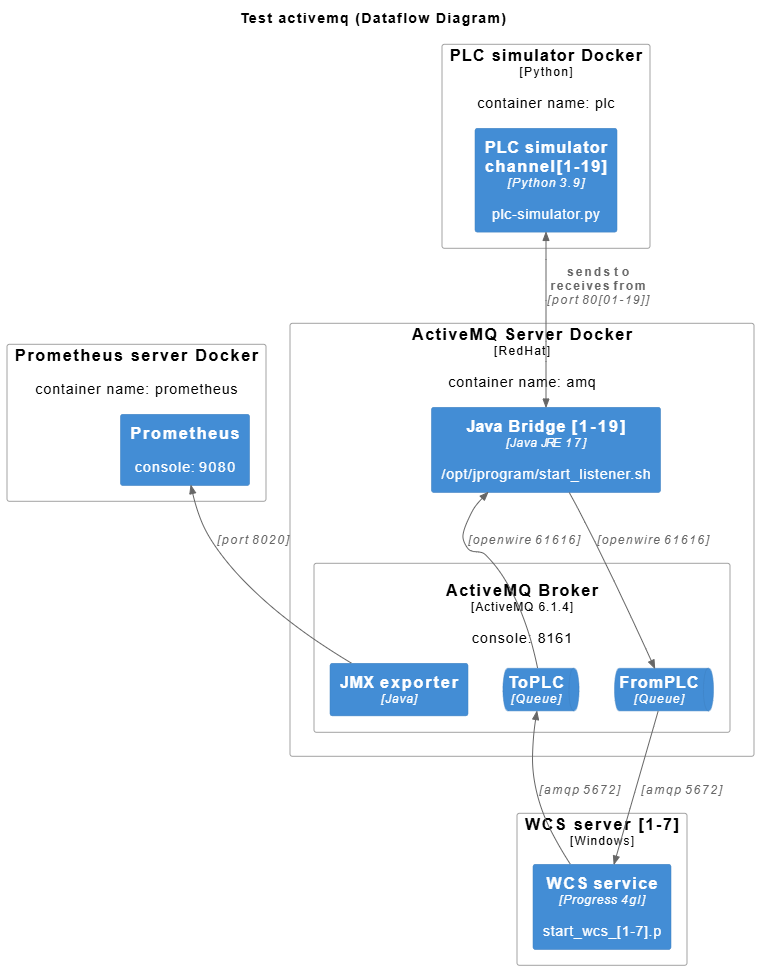
\includegraphics[width=.5\textwidth]{img/test_amq_dataflow.png}
  \caption{\label{fig:test_amq_dataflow}Dataflow test AMQ}
\end{figure}

DockerFile

\subsection{Test RabbitMQ}
Overzicht van de infrastructuur:
\begin{figure}[h!]
  \centering
  \includegraphics[width=.5\textwidth]{img/test_rabbitmq_dataflow.png}
  \caption{\label{fig:test_rabbitmq_dataflow}Dataflow test RabbitMQ}
\end{figure}

\subsection{Test Artemis}
Overzicht van de infrastructuur:
\begin{figure}[h!]
  \centering
  \includegraphics[width=.5\textwidth]{img/test_artemis_dataflow.png}
  \caption{\label{fig:test_artemis_dataflow}Dataflow test Artemis}
\end{figure}









